En este capítulo se explican y detallan las etapas que permiten modelar la solución propuesta utilizando artefactos de \textit{software}, que permiten documentar el sistema bajo el marco de trabajo de una metodología de desarrollo de \textit{software}.


\subsection{Metodología}

Una metodología de desarrollo de \textit{software} puede ser definida como un marco de trabajo que se utiliza para estructurar, planificar y controlar el proceso correspondiente al desarrollo de un sistema de información. Para una administración y gestión sistemática de todo proyecto de \textit{software}, y llevarlo a cabo con altas posibilidades de éxito, es necesario guiarse por una metodología, permitiendo así dividir un proyecto en módulos o etapas. De esta forma estructurada y organizada es posible crear, desarrollar y mantener un sistema desde que surge la necesidad del producto hasta que se cumple el objetivo por el cual fue desarrollado.\\

En este proyecto se utilizará el ciclo de vida incremental para el desarrollo del \textit{software}, ya que este modelo se acomoda bastante a la implementación de un prototipo, que es el caso de este proyecto de tesis. Además, no es necesario disponer de los requerimientos de todas las funcionalidades en el comienzo del mismo. El proceso consiste en ir construyendo módulos o iteraciones que van cumpliendo con las diferentes funciones del sistema, aumentando gradualmente las capacidades de éste. Las ventajas de este ciclo de vida son:

\begin{enumerate}
\item Desarrollar las funcionalidades por etapas permite detectar si los requerimientos planteados para los niveles siguientes son correctos.
\item En caso de enfrentarse ante un error grave solo se desecha la última iteración.
\item Construir por etapas, partes pequeñas del sistema, representa menos riesgo que construir un sistema grande.
\end{enumerate}


\subsection{Plan de trabajo}

En la Figura 10 se ilustra el plan de trabajo para llevar a cabo la implementación del sistema:

\begin{figure}[H]
\centering
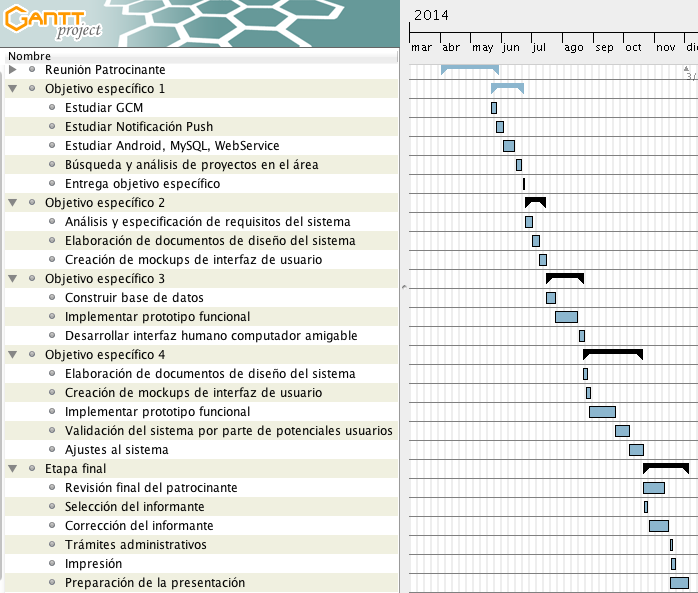
\includegraphics[scale=0.65]{images/capitulo4/gantt.png}
\caption{Carta Gantt que exhibe las etapas de desarrollo del sistema.}
\label{gantt}
\end{figure}


\subsubsection{Estrategia de implementación}

A través del proceso de implementación y desarrollo del software, se tuvo que tomar en cuenta lo siguiente:

\begin{enumerate}
\item Es importante reunirse con el profesor patrocinante al comienzo, durante y al término de una iteración, para así aclarar y resolver requerimientos específicos del sistema que puedan surgir.
\item Durante el desarrollo del sistema, se consideran presentaciones de avance de las iteraciones de tal forma que se disminuyan errores y/o riesgos en la entrega final.
\item El producto final se dará terminado cuando se hayan cumplido todos los requisitos del sistema.
\end{enumerate}

\subsection{Análisis}

\subsubsection{Descripción de los actores del sistema}

\textbf{Administrador:} es un individuo que se ocupa de configurar el sistema, antes de la puesta en marcha, y tiene acceso a todas las funcionalidades del mismo. Es decir, es un funcionario del centro de atención donde sea instalado el sistema de gestión de tickets.\\

\textbf{Ejecutivo:} es un funcionario del centro de atención que utilza el sistema para realizar las llamadas a los clientes cuando sea oportuno. Tiene acceso limitado a la aplicación web.\\

\textbf{Cliente:} corresponde a una persona que interactúa como cliente con el sistema a través de la aplicación móvil desde su \textit{smartphone} en un centro de atención. \\

\subsubsection{Casos de Uso}

\begin{figure}[H]
\centering
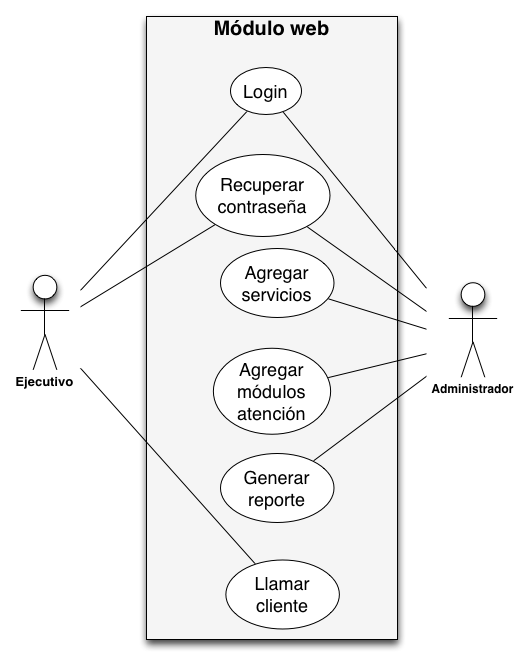
\includegraphics[scale=0.65]{images/capitulo4/moduloWeb.png}
\caption{Diagrama de Casos de Uso Módulo web.}
\label{cuModuloWeb}
\end{figure}

\begin{figure}[H]
\centering
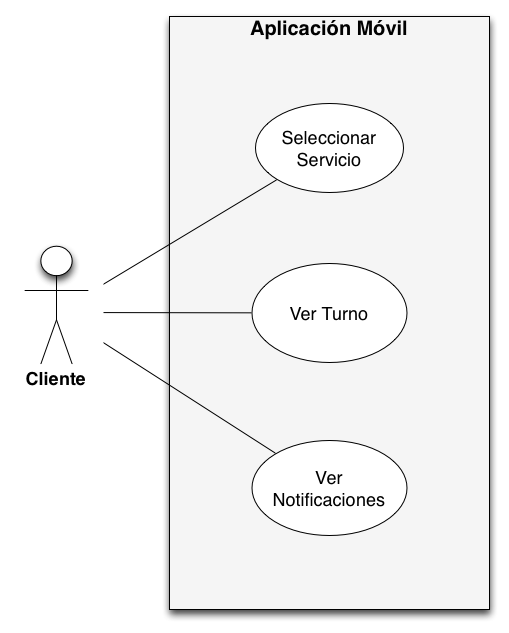
\includegraphics[scale=0.60]{images/capitulo4/appMovil.png}
\caption{Diagrama de Casos de Uso Aplicación Móvil.}
\label{cuAppMovil}
\end{figure}

\subsection{Especificación de requerimientos}

De acuerdo a la problemática y objetivos descritos se tomaron y obtuvieron los requisitos para poder desarrollar el Sistema de Gestión de tickes de espera.

\subsubsection{Requisitos Funcionales}

Cuando se plantea una solución a una problemática, nacen ideas de cómo será y qué características tendrá el sistema que se desarrollará. Éstas características requeridas del \textit{software} tienen relación con una capacidad de acción que tendrá el nuevo sistema, es decir, una funcionalidad.\\ 

A continuación en la tabla 3 se presentan los requisitos funcionales extraídos de los diagramas UML y de las capacidades que se desea que tenga el sistema a implementar.

\begin{spacing}{1.0}
\begin{table}[H]
\centering
\caption{Requisitos Funcionales.} 
\begin{tabular}{|c|c|}
\hline 
\rowcolor{gray!30} &\\
\rowcolor{gray!30} \textbf{Ref. \#} & \textbf{Función} \\ 
\rowcolor{gray!30} &\\
\hline 
&\\[-0.2cm]
FRQ-001 & Iniciar sesión en aplicación web.\\
\hline
&\\[-0.2cm]
FRQ-002 & Cargar y mostrar servicios.\\
\hline
&\\[-0.2cm]
FRQ-003 & Cargar y mostrar módulos de atención.\\
\hline
&\\[-0.2cm]
FRQ-004 & Enviar notificaciones desde aplicación web a \textit{smartphone}.\\ 
\hline
&\\[-0.2cm]
FRQ-005 & Generar reportes.\\
\hline
&\\[-0.2cm]
FRQ-006 & Mostrar últimos turnos en atención.\\
\hline
&\\[-0.2cm]
FRQ-007 & Monitor de atenciones.\\
\hline
&\\[-0.2cm]
FRQ-008 & Mostrar servicios.\\
\hline
&\\[-0.2cm]
FRQ-009 & Selecionar un servicio.\\ 
\hline
&\\[-0.2cm]
FRQ-010 & Ver turno de atención.\\
\hline
&\\[-0.2cm]
FRQ-011 & Ver notificaciones.\\
\hline
&\\[-0.2cm]
FRQ-012 & Mostrar notificaciones nuevas automáticamente.\\
\hline
&\\[-0.2cm]
FRQ-013 & Mostrar información de la aplicación.\\
\hline
\end{tabular}
\label{tabla_pila}
\end{table}
\end{spacing}

\subsubsection{Requisitos No Funcionales}

Los requisitos no funcionales, obedecen a todas las exigencias cualitativas que se imponen, es decir, cómo debe ser el sistema. Generalmente corresponden a requisitos que son restricciones que se deben cumplir y que se encuentran fuera del conjunto de los requisitos funcionales. A continuación en la tabla 4 se especifican los requisitos no funcionales del sistema.

\begin{spacing}{1.0}
\begin{table}[H]
\centering
\caption{Requisitos No Funcionales.} 
\begin{tabular}{|c|c|}
\hline 
\rowcolor{gray!30} &\\
\rowcolor{gray!30} \textbf{Ref. \#} & \textbf{Función} \\ 
\rowcolor{gray!30} &\\
\hline 
&\\[-0.2cm]
FRQ-014 & Interfaz del sistema debe ser amigable con el usuario.\\
\hline
&\\[-0.2cm]
FRQ-015 & Bajo tráfico de datos.\\
\hline
&\\[-0.2cm]
FRQ-016 & Portabilidad.\\
\hline
&\\[-0.2cm]
FRQ-017 & La aplicación móvil debe ser desarrollada para Android.\\
\hline
\end{tabular}
\label{tabla_pila}
\end{table}
\end{spacing}



\myparagraph{Casos de Uso Extendido del sistema}


\begin{spacing}{1.0}
	\begin{table}[H]
		\centering
		\caption{Caso de uso extendido ``Agregar Servicios''.} 
		\begin{tabular}{| >{\arraybackslash\columncolor{gray!30}}p{3.1cm}| >{\arraybackslash}p{10.4cm}|}
			\hline 
			\rowcolor{gray!30} &\\[-0.2cm]
			\rowcolor{gray!30} \textbf{Caso de uso:} & \textbf{Agregar Servicios (CU01).} \\[0.2cm]
			\hline
			&\\[-0.2cm]
			\textbf{Actores:} & Administrador. \\[0.2cm]
			\hline
			&\\[-0.2cm]
			\textbf{Propósito:} & Agregar servicios al sistema. \\[0.2cm]
			\hline
			&\\[-0.2cm]
			\textbf{Resumen:} & El Administrador agrega todos los servicios que brinda el centro de atención, a la base de datos ubicada en el servidor central. \\[0.2cm]
			\hline
			&\\[-0.2cm]
			\textbf{Tipo:} & Primario y esencial. \\[0.2cm]
			\hline
			&\\[-0.2cm]
			\textbf{Precondiciones:} & {\tiny$\blacksquare$} La base de datos, servidor web y servidor central deben estar operativos. \\[0.2cm]
			\hline
			\multicolumn{2}{| >{\arraybackslash\columncolor{gray!30}}c|}{}\\[-0.2cm]
			\multicolumn{2}{| >{\arraybackslash\columncolor{gray!30}}c|}{\textbf{Curso normal de los eventos}}\\[0.2cm]
		\end{tabular}
		
		\vspace{-0.5cm}
		\begin{center}
			\begin{tabular}{| >{\arraybackslash}p{6.75cm} | >{\arraybackslash}p{6.75cm} |}
				\hline
				\rowcolor{gray!30} &\\[-0.2cm]
				\rowcolor{gray!30} \textbf{Acción de los actores} & \textbf{Respuesta del sistema}\\[0.2cm]
				\hline
				&\\[-0.2cm]
				\textbf{1.} Este caso de uso comienza cuando se debe preparar el sistema para ser utilizado en el centro de atención. & \\
				\textbf{2.} El Administrador se dirige a la opción que le permite agregar un servicio. &\\
				& \textbf{3.} Muestra la interfaz para realizar esta acción. \\
				\textbf{4.} El Administrador ingresa el nombre del servicio y agrega el servicio al sistema. & \\
				& \textbf{5.} La base de datos recibe y graba la información. \\
				& \textbf{6.} El servicio es agregado y se muestra en la ventana. \\
				\hline
				\multicolumn{2}{| >{\arraybackslash\columncolor{gray!30}}c|}{}\\[-0.2cm]
				\multicolumn{2}{| >{\arraybackslash\columncolor{gray!30}}c|}{\textbf{Cursos alternativos}}\\[0.2cm]
				\hline
				\multicolumn{2}{|l|}{}\\[-0.2cm]
				\multicolumn{2}{|l|}{\textbf{4.} El servicio ya existe.}\\
				\multicolumn{2}{|l|}{\textbf{5.} El sistema no responde ante el envío de los datos.}\\
			\end{tabular}
		\end{center}
		
		\vspace{-0.5cm}
		\begin{tabular}{| >{\arraybackslash\columncolor{gray!30}}p{3.1cm}| >{\arraybackslash}p{10.4cm}|}
			\hline
			&\\[-0.2cm]
			\textbf{Post condiciones:} & El sistema queda esperando para repetir el proceso o realizar uno diferente. \\[0.2cm]
			\hline
		\end{tabular}
		
		\label{tabla_CU01}
	\end{table}
\end{spacing}


\begin{spacing}{1.0}
	\begin{table}[H]
		\centering
		\caption{Caso de uso extendido ``Agregar Módulo Atención''.} 
		\begin{tabular}{| >{\arraybackslash\columncolor{gray!30}}p{3.1cm}| >{\arraybackslash}p{10.4cm}|}
			\hline 
			\rowcolor{gray!30} &\\[-0.2cm]
			\rowcolor{gray!30} \textbf{Caso de uso:} & \textbf{Agregar Módulo Atención (CU02).} \\[0.2cm]
			\hline
			&\\[-0.2cm]
			\textbf{Actores:} & Administrador. \\[0.2cm]
			\hline
			&\\[-0.2cm]
			\textbf{Propósito:} & Agregar módulos de atencion al sistema. \\[0.2cm]
			\hline
			&\\[-0.2cm]
			\textbf{Resumen:} & El Administrador agrega tal sistema todos los módulos donde se atenderán clientes. \\[0.2cm]
			\hline
			&\\[-0.2cm]
			\textbf{Tipo:} & Primario y esencial. \\[0.2cm]
			\hline
			&\\[-0.2cm]
			\textbf{Precondiciones:} & {\tiny$\blacksquare$} La base de datos, servidor web y servidor central deben estar operativos. \\[0.2cm]
			\hline
			\multicolumn{2}{| >{\arraybackslash\columncolor{gray!30}}c|}{}\\[-0.2cm]
			\multicolumn{2}{| >{\arraybackslash\columncolor{gray!30}}c|}{\textbf{Curso normal de los eventos}}\\[0.2cm]
		\end{tabular}
		
		\vspace{-0.5cm}
		\begin{center}
			\begin{tabular}{| >{\arraybackslash}p{6.75cm} | >{\arraybackslash}p{6.75cm} |}
				\hline
				\rowcolor{gray!30} &\\[-0.2cm]
				\rowcolor{gray!30} \textbf{Acción de los actores} & \textbf{Respuesta del sistema}\\[0.2cm]
				\hline
				&\\[-0.2cm]
				\textbf{1.} Este caso de uso comienza luego de que el Administrador haya ingresado los servicios (CU01). & \\
				\textbf{2.} El Administrador se dirige a la opción que le permite agregar un módulo de atención. &\\
				& \textbf{3.} Muestra la interfaz para realizar esta acción. \\
				\textbf{4.} El Administrador ingresa el nombre del módulo de atención y lo agrega al sistema. & \\
				& \textbf{5.} La base de datos recibe y graba la información. \\
				& \textbf{6.} El módulo de atención es agregado y se muestra en la ventana. \\
				\hline
				\multicolumn{2}{| >{\arraybackslash\columncolor{gray!30}}c|}{}\\[-0.2cm]
				\multicolumn{2}{| >{\arraybackslash\columncolor{gray!30}}c|}{\textbf{Cursos alternativos}}\\[0.2cm]
				\hline
				\multicolumn{2}{|l|}{}\\[-0.2cm]
				\multicolumn{2}{|l|}{\textbf{4.} El módulo de atención ya existe.}\\
				\multicolumn{2}{|l|}{\textbf{5.} El sistema no responde ante el envío de los datos.}\\
			\end{tabular}
		\end{center}
		
		\vspace{-0.5cm}
		\begin{tabular}{| >{\arraybackslash\columncolor{gray!30}}p{3.1cm}| >{\arraybackslash}p{10.4cm}|}
			\hline
			&\\[-0.2cm]
			\textbf{Post condiciones:} & El sistema queda esperando para repetir el proceso o realizar uno diferente. \\[0.2cm]
			\hline
		\end{tabular}
		
		\label{tabla_CU02}
	\end{table}
\end{spacing}

\begin{spacing}{1.0}
	\begin{table}[H]
		\centering
		\caption{Caso de uso extendido ``Seleccionar Servicio''.} 
		\begin{tabular}{| >{\arraybackslash\columncolor{gray!30}}p{3.1cm}| >{\arraybackslash}p{10.4cm}|}
			\hline 
			\rowcolor{gray!30} &\\[-0.2cm]
			\rowcolor{gray!30} \textbf{Caso de uso:} & \textbf{Seleccionar Servicio (CU03).} \\[0.2cm]
			\hline
			&\\[-0.2cm]
			\textbf{Actores:} & Cliente. \\[0.2cm]
			\hline
			&\\[-0.2cm]
			\textbf{Propósito:} & Obtener un turno de atención. \\[0.2cm]
			\hline
			&\\[-0.2cm]
			\textbf{Resumen:} & El usuario se abre la aplicación \textbf{Mi Turno} y presiona un servicio, mostrado en la pantalla principal, para obtener un turno de atención. \\[0.2cm]
			\hline
			&\\[-0.2cm]
			\textbf{Tipo:} & Primario y esencial. \\[0.2cm]
			\hline
			&\\[-0.2cm]
			\textbf{Precondiciones:} & {\tiny$\blacksquare$} El dispositivo móvil debe tener conexión a Internet. \\
			& {\tiny$\blacksquare$} La base de datos, servidor web y servidor central deben estar operativos. \\ [0.2cm]
			\hline
			\multicolumn{2}{| >{\arraybackslash\columncolor{gray!30}}c|}{}\\[-0.2cm]
			\multicolumn{2}{| >{\arraybackslash\columncolor{gray!30}}c|}{\textbf{Curso normal de los eventos}}\\[0.2cm]
		\end{tabular}
		
		\vspace{-0.5cm}
		\begin{center}
			\begin{tabular}{| >{\arraybackslash}p{6.75cm} | >{\arraybackslash}p{6.75cm} |}
				\hline
				\rowcolor{gray!30} &\\[-0.2cm]
				\rowcolor{gray!30} \textbf{Acción de los actores} & \textbf{Respuesta del sistema}\\[0.2cm]
				\hline
				&\\[-0.2cm]
				\textbf{1.} Este caso de uso comienza cuando un Cliente se acerca a un centro de atención y, desea obtener un turno para realizar un trámite en algún servicio del centro de atención. & \\
				\textbf{2.} El Cliente presiona un botón correspondiente al servicio que desea. &\\
				& \textbf{3.} Muestra un cuadro de diálogo donde pregunta \textbf{¿Desea obtener ticket de atención?}. \\
				& \textbf{5.} Muestra un mensaje confirmando la acción. \\
				&\textbf{6.} Muestra una nueva pantalla donde se indica el \textbf{Turno} y \textbf{Servicio}. \\
				\hline
				\multicolumn{2}{| >{\arraybackslash\columncolor{gray!30}}c|}{}\\[-0.2cm]
				\multicolumn{2}{| >{\arraybackslash\columncolor{gray!30}}c|}{\textbf{Cursos alternativos}}\\[0.2cm]
				\hline
				\multicolumn{2}{|l|}{}\\[-0.2cm]
				\multicolumn{2}{|l|}{\textbf{4.} El Cliente presionó equivocadamente el servicio y presiona el botón \textbf{NO}.}\\
				\multicolumn{2}{|l|}{\textbf{5.} El dispositivo móvil pierde comunicación con el servidor central.}\\
			\end{tabular}
		\end{center}
		
		\vspace{-0.5cm}
		\begin{tabular}{| >{\arraybackslash\columncolor{gray!30}}p{3.1cm}| >{\arraybackslash}p{10.4cm}|}
			\hline
			&\\[-0.2cm]
			\textbf{Post condiciones:} & La aplicación móvil queda trabajando en segundo plano a la espera de recibir Notificaciones. \\[0.2cm]
			\hline
		\end{tabular}
		
		\label{tabla_CU03}
	\end{table}
\end{spacing}

\subsection{Diseño}

\subsubsection{Casos de Uso Real}

\begin{spacing}{1.0}
	\begin{table}[H]
		\centering
		\caption{Caso de uso Real ``Agregar Servicios''.} 
		\begin{tabular}{| >{\arraybackslash\columncolor{gray!30}}p{3.1cm}| >{\arraybackslash}p{10.4cm}|}
			\hline 
			\rowcolor{gray!30} &\\[-0.2cm]
			\rowcolor{gray!30} \textbf{Caso de uso:} & \textbf{Agregar Servicios (CU01).} \\[0.2cm]
			\hline
			&\\[-0.2cm]
			\textbf{Actores:} & Administrador. \\[0.2cm]
			\hline
			&\\[-0.2cm]
			\textbf{Propósito:} & Agregar servicios al sistema. \\[0.2cm]
			\hline
			&\\[-0.2cm]
			\textbf{Resumen:} & El Administrador agrega todos los servicios que brinda el centro de atención, a la base de datos ubicada en el servidor central. \\[0.2cm]
			\hline
			&\\[-0.2cm]
			\textbf{Tipo:} & Primario y esencial. \\[0.2cm]
			\hline
			&\\[-0.2cm]
			\textbf{Precondiciones:} & {\tiny$\blacksquare$} La base de datos, servidor web y servidor central deben estar operativos. \\[0.2cm]
			\hline
			\multicolumn{2}{| >{\arraybackslash\columncolor{gray!30}}c|}{}\\[-0.2cm]
			\multicolumn{2}{| >{\arraybackslash\columncolor{gray!30}}c|}{\textbf{Curso normal de los eventos}}\\[0.2cm]
		\end{tabular}
		
		\vspace{-0.5cm}
		\begin{center}
			\begin{tabular}{| >{\arraybackslash}p{6.75cm} | >{\arraybackslash}p{6.75cm} |}
				\hline
				\rowcolor{gray!30} &\\[-0.2cm]
				\rowcolor{gray!30} \textbf{Acción de los actores} & \textbf{Respuesta del sistema}\\[0.2cm]
				\hline
				&\\[-0.2cm]
				\textbf{1.} Este caso de uso comienza cuando se debe preparar el sistema para ser utilizado en el centro de atención. & \\
				\textbf{2.} El Administrador se dirige a la opción \textbf{Configuración} \textbf{(A)}, luego a \textbf{Agregar Servicios} \textbf{(B)}. &\\
				& \textbf{3.} Muestra la interfaz para realizar esta acción. \\
				\textbf{4.} El Administrador ingresa el nombre del servicio en la entrada de texto \textbf{(C)} y presiona el boton \textbf{Agregar} \textbf{(D)}. & \\
				& \textbf{5.} La base de datos recibe y graba la información. \\
				& \textbf{6.} El servicio es agregado y se muestra en la lista de servicios \textbf{(E)}. \\
				\hline
				\multicolumn{2}{| >{\arraybackslash\columncolor{gray!30}}c|}{}\\[-0.2cm]
				\multicolumn{2}{| >{\arraybackslash\columncolor{gray!30}}c|}{\textbf{Cursos alternativos}}\\[0.2cm]
				\hline
				\multicolumn{2}{|l|}{}\\[-0.2cm]
				\multicolumn{2}{|l|}{\textbf{4.} El servicio ya existe.}\\
				\multicolumn{2}{|l|}{\textbf{5.} El sistema no responde ante el envío de los datos.}\\
			\end{tabular}
		\end{center}
		
		\vspace{-0.5cm}
		\begin{tabular}{| >{\arraybackslash\columncolor{gray!30}}p{3.1cm}| >{\arraybackslash}p{10.4cm}|}
			\hline
			&\\[-0.2cm]
			\textbf{Post condiciones:} & El sistema queda esperando para repetir el proceso o realizar uno diferente. \\[0.2cm]
			\hline
		\end{tabular}
		
		\label{tabla_CU01}
	\end{table}
\end{spacing}

\begin{figure}[H]
\centering
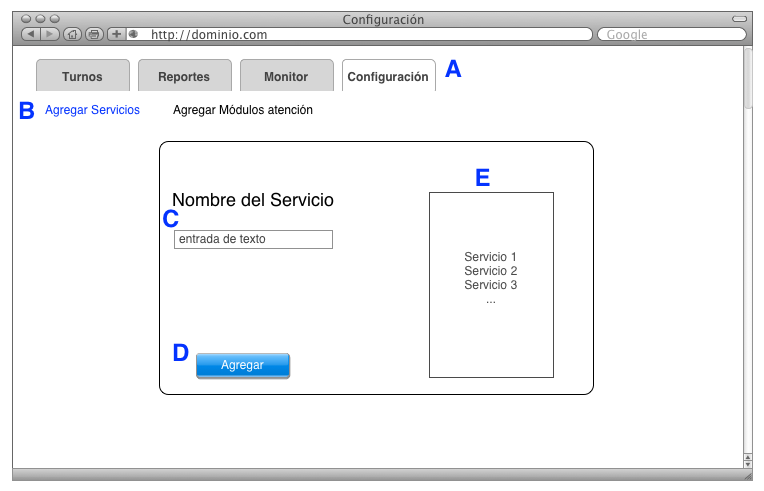
\includegraphics[scale=0.55]{images/capitulo4/mockupCU01.png}
\caption{\textit{Mockup} Caso de Uso 1 (CU01).}
\label{mockupCU01}
\end{figure}


\begin{spacing}{1.0}
	\begin{table}[H]
		\centering
		\caption{Caso de uso Real ``Agregar Módulo Atención''.} 
		\begin{tabular}{| >{\arraybackslash\columncolor{gray!30}}p{3.1cm}| >{\arraybackslash}p{10.4cm}|}
			\hline 
			\rowcolor{gray!30} &\\[-0.2cm]
			\rowcolor{gray!30} \textbf{Caso de uso:} & \textbf{Agregar Módulo Atención (CU02).} \\[0.2cm]
			\hline
			&\\[-0.2cm]
			\textbf{Actores:} & Administrador. \\[0.2cm]
			\hline
			&\\[-0.2cm]
			\textbf{Propósito:} & Agregar módulos de atencion al sistema. \\[0.2cm]
			\hline
			&\\[-0.2cm]
			\textbf{Resumen:} & El Administrador agrega tal sistema todos los módulos donde se atenderán clientes. \\[0.2cm]
			\hline
			&\\[-0.2cm]
			\textbf{Tipo:} & Primario y esencial. \\[0.2cm]
			\hline
			&\\[-0.2cm]
			\textbf{Precondiciones:} & {\tiny$\blacksquare$} La base de datos, servidor web y servidor central deben estar operativos. \\[0.2cm]
			\hline
			\multicolumn{2}{| >{\arraybackslash\columncolor{gray!30}}c|}{}\\[-0.2cm]
			\multicolumn{2}{| >{\arraybackslash\columncolor{gray!30}}c|}{\textbf{Curso normal de los eventos}}\\[0.2cm]
		\end{tabular}
		
		\vspace{-0.5cm}
		\begin{center}
			\begin{tabular}{| >{\arraybackslash}p{6.75cm} | >{\arraybackslash}p{6.75cm} |}
				\hline
				\rowcolor{gray!30} &\\[-0.2cm]
				\rowcolor{gray!30} \textbf{Acción de los actores} & \textbf{Respuesta del sistema}\\[0.2cm]
				\hline
				&\\[-0.2cm]
				\textbf{1.} Este caso de uso comienza luego de que el Administrador haya ingresado los servicios (CU01). & \\
				\textbf{2.} El Administrador se dirige a la opción \textbf{Configuración} \textbf{(A)}, luego a \textbf{Agregar Servicios} \textbf{(B)}. &\\
				& \textbf{3.} Muestra la interfaz para realizar esta acción. \\
				\textbf{4.} El Administrador ingresa el nombre del módulo de atención en la entrada de texto \textbf{(C)} y presiona el boton \textbf{Agregar} \textbf{(D)}. & \\
				& \textbf{5.} La base de datos recibe y graba la información. \\
				& \textbf{6.} El módulo de atención es agregado y se muestra en la lista de servicios \textbf{(E)} \\
				\hline
				\multicolumn{2}{| >{\arraybackslash\columncolor{gray!30}}c|}{}\\[-0.2cm]
				\multicolumn{2}{| >{\arraybackslash\columncolor{gray!30}}c|}{\textbf{Cursos alternativos}}\\[0.2cm]
				\hline
				\multicolumn{2}{|l|}{}\\[-0.2cm]
				\multicolumn{2}{|l|}{\textbf{4.} El módulo de atención ya existe.}\\
				\multicolumn{2}{|l|}{\textbf{5.} El sistema no responde ante el envío de los datos.}\\
			\end{tabular}
		\end{center}
		
		\vspace{-0.5cm}
		\begin{tabular}{| >{\arraybackslash\columncolor{gray!30}}p{3.1cm}| >{\arraybackslash}p{10.4cm}|}
			\hline
			&\\[-0.2cm]
			\textbf{Post condiciones:} & El sistema queda esperando para repetir el proceso o realizar uno diferente. \\[0.2cm]
			\hline
		\end{tabular}
		
		\label{tabla_CU02}
	\end{table}
\end{spacing}

\begin{figure}[H]
\centering
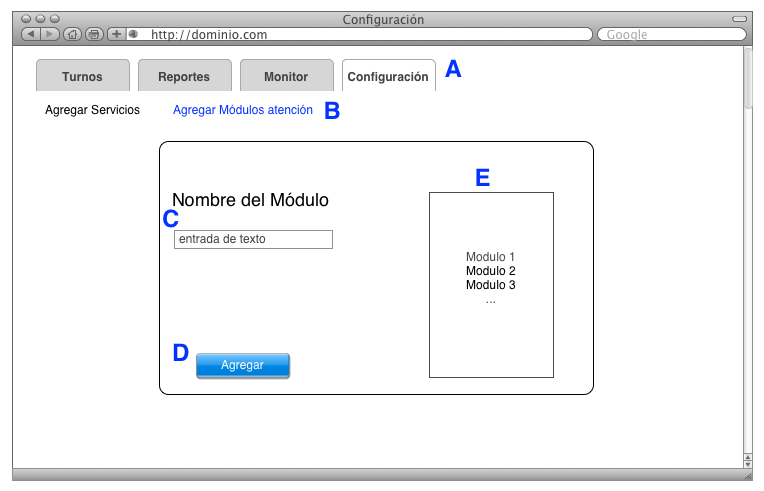
\includegraphics[scale=0.55]{images/capitulo4/mockupCU02.png}
\caption{\textit{Mockup} Caso de Uso 2 (CU02).}
\label{mockupCU01}
\end{figure}

\begin{spacing}{1.0}
	\begin{table}[H]
		\centering
		\caption{Caso de uso Real ``Seleccionar Servicio''.} 
		\begin{tabular}{| >{\arraybackslash\columncolor{gray!30}}p{3.1cm}| >{\arraybackslash}p{10.4cm}|}
			\hline 
			\rowcolor{gray!30} &\\[-0.2cm]
			\rowcolor{gray!30} \textbf{Caso de uso:} & \textbf{Seleccionar Servicio (CU03).} \\[0.2cm]
			\hline
			&\\[-0.2cm]
			\textbf{Actores:} & Cliente. \\[0.2cm]
			\hline
			&\\[-0.2cm]
			\textbf{Propósito:} & Obtener un turno de atención. \\[0.2cm]
			\hline
			&\\[-0.2cm]
			\textbf{Resumen:} & El usuario se abre la aplicación \textbf{Mi Turno} y presiona un servicio, mostrado en la pantalla principal, para obtener un turno de atención. \\[0.2cm]
			\hline
			&\\[-0.2cm]
			\textbf{Tipo:} & Primario y esencial. \\[0.2cm]
			\hline
			&\\[-0.2cm]
			\textbf{Precondiciones:} & {\tiny$\blacksquare$} El dispositivo móvil debe tener conexión a Internet. \\
			& {\tiny$\blacksquare$} La base de datos, servidor web y servidor central deben estar operativos. \\ [0.2cm]
			\hline
			\multicolumn{2}{| >{\arraybackslash\columncolor{gray!30}}c|}{}\\[-0.2cm]
			\multicolumn{2}{| >{\arraybackslash\columncolor{gray!30}}c|}{\textbf{Curso normal de los eventos}}\\[0.2cm]
		\end{tabular}
		
		\vspace{-0.5cm}
		\begin{center}
			\begin{tabular}{| >{\arraybackslash}p{6.75cm} | >{\arraybackslash}p{6.75cm} |}
				\hline
				\rowcolor{gray!30} &\\[-0.2cm]
				\rowcolor{gray!30} \textbf{Acción de los actores} & \textbf{Respuesta del sistema}\\[0.2cm]
				\hline
				&\\[-0.2cm]
				\textbf{1.} Este caso de uso comienza cuando un Cliente se acerca a un centro de atención y, desea obtener un turno para realizar un trámite en algún servicio del centro de atención. & \\
				\textbf{2.} El Cliente presiona un botón correspondiente al servicio que desea \textbf{(A)}. &\\
				& \textbf{3.} Muestra un cuadro de diálogo donde pregunta \textbf{¿Desea obtener ticket de atención?} \textbf{(B)}. \\
				\textbf{4.} El Cliente en caso que desee ese servicio presiona el botón \textbf{SI} \textbf{(C)}.  \\
				& \textbf{5.} Muestra un mensaje confirmando la acción. \\
				&\textbf{6.} Muestra una nueva pantalla donde se indica el \textbf{Turno} y \textbf{Servicio} \textbf{(D)}. \\
				\hline
				\multicolumn{2}{| >{\arraybackslash\columncolor{gray!30}}c|}{}\\[-0.2cm]
				\multicolumn{2}{| >{\arraybackslash\columncolor{gray!30}}c|}{\textbf{Cursos alternativos}}\\[0.2cm]
				\hline
				\multicolumn{2}{|l|}{}\\[-0.2cm]
				\multicolumn{2}{|l|}{\textbf{4.} El Cliente presionó equivocadamente el servicio y presiona el botón \textbf{NO}.}\\
				\multicolumn{2}{|l|}{\textbf{5.} El dispositivo móvil pierde comunicación con el servidor central.}\\
			\end{tabular}
		\end{center}
		
		\vspace{-0.5cm}
		\begin{tabular}{| >{\arraybackslash\columncolor{gray!30}}p{3.1cm}| >{\arraybackslash}p{10.4cm}|}
			\hline
			&\\[-0.2cm]
			\textbf{Post condiciones:} & La aplicación móvil queda trabajando en segundo plano a la espera de recibir Notificaciones. \\[0.2cm]
			\hline
		\end{tabular}
		
		\label{tabla_CU03}
	\end{table}
\end{spacing}

\begin{figure}[H]
\centering
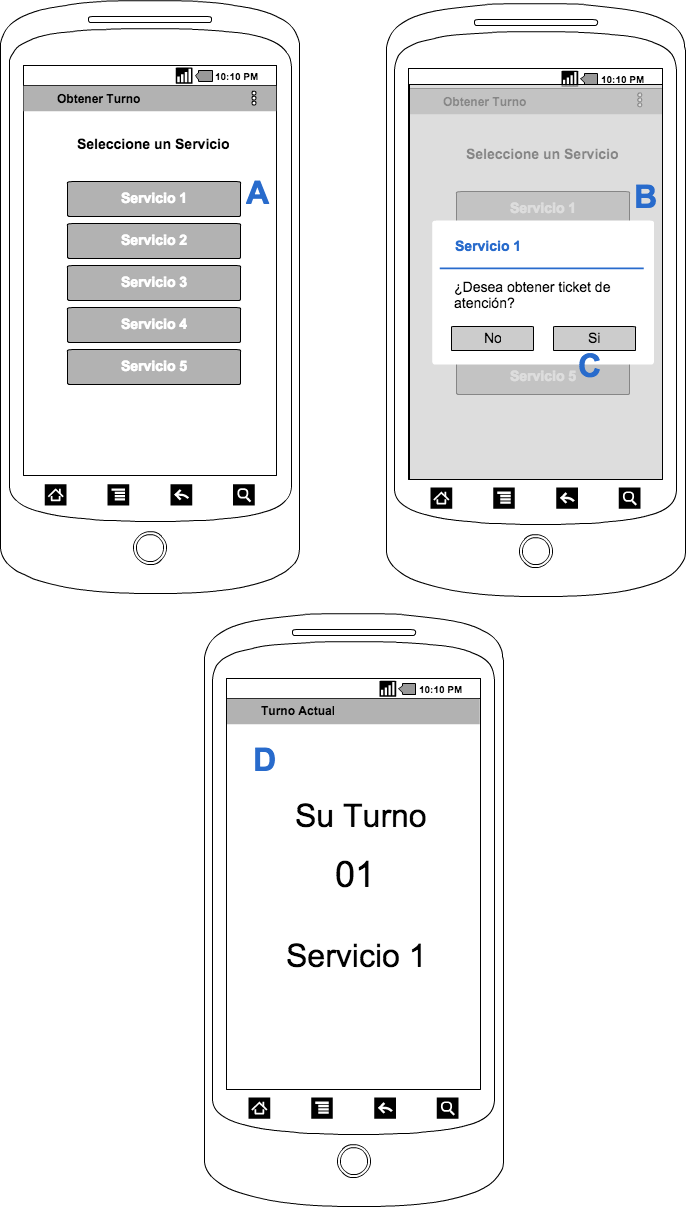
\includegraphics[scale=0.40]{images/capitulo4/mockupCU03.png}
\caption{\textit{Mockup} Caso de Uso 3 (CU03).}
\label{mockupCU03}
\end{figure}


\subsubsection{Diagramas de Secuencia}

\begin{figure}[H]
\centering
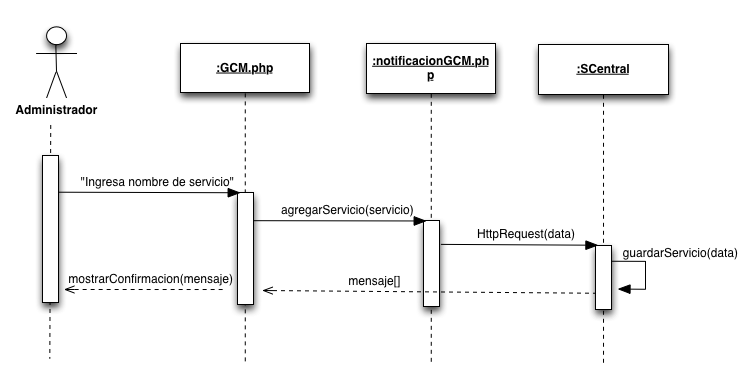
\includegraphics[scale=0.65]{images/capitulo4/dsAgregarServicio.png}
\caption{Diagrama de Secuencia Caso de Uso Agregar Servicios.}
\label{dsCUAS}
\end{figure}

\begin{figure}[H]
\centering
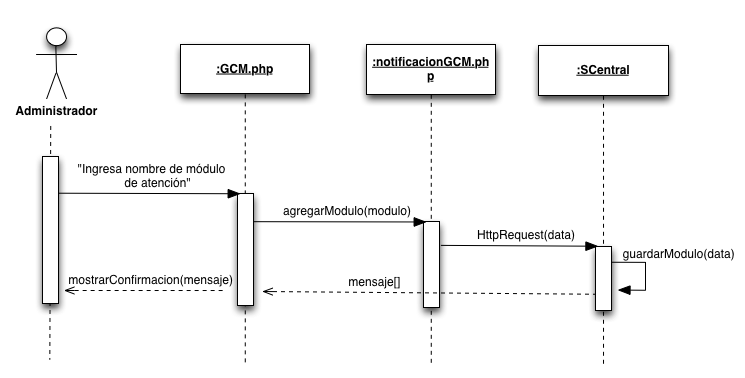
\includegraphics[scale=0.65]{images/capitulo4/dsAgregarModulo.png}
\caption{Diagrama de Secuencia Caso de Uso Agregar Módulo Atención.}
\label{dsCUAMA}
\end{figure}

\begin{figure}[H]
\centering
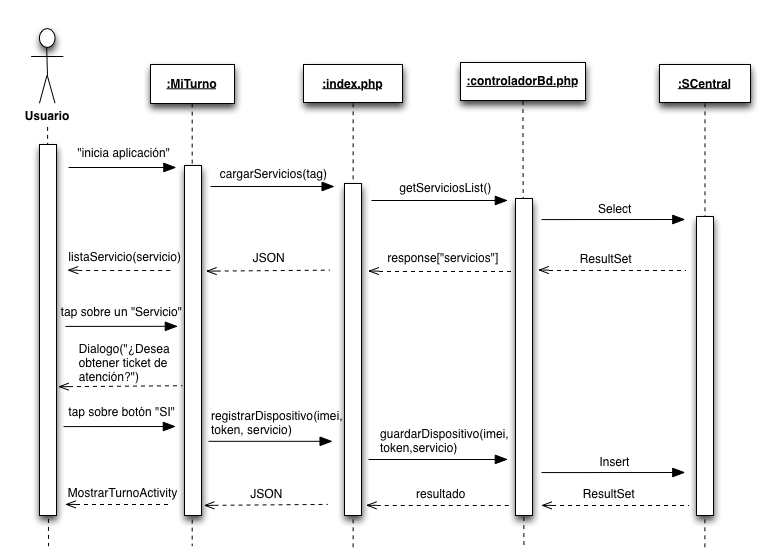
\includegraphics[scale=0.60]{images/capitulo4/dsSeleccionarServicio.png}
\caption{Diagrama de Secuencia Caso de Uso Seleccionar Servicio.}
\label{dsCUSS}
\end{figure}

\subsubsection{Diagrama de Clases}

\begin{figure}[H]
\centering
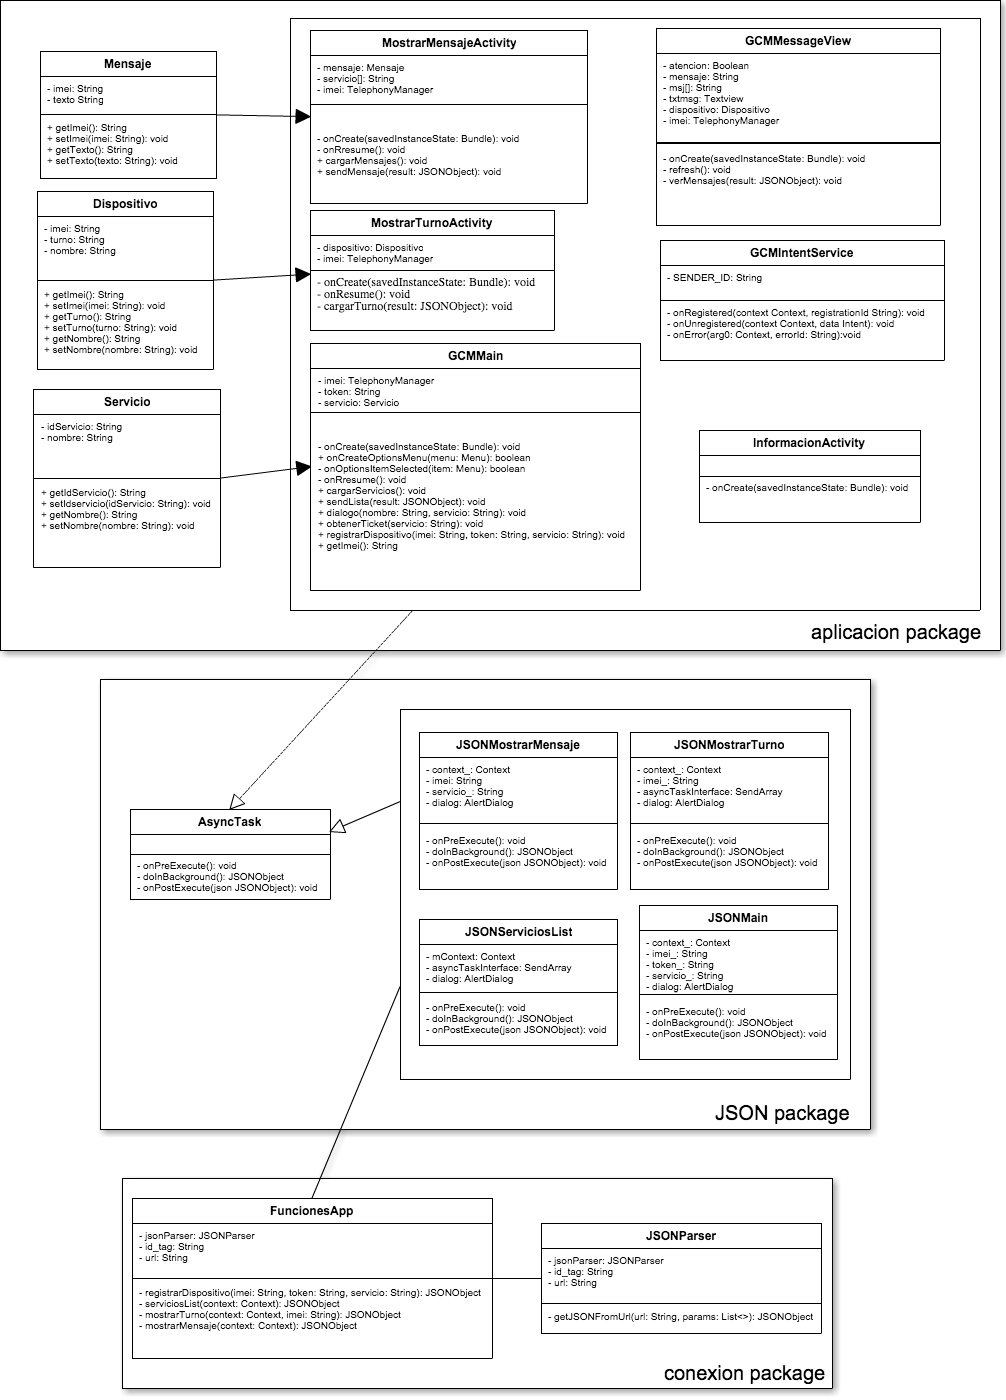
\includegraphics[scale=0.45]{images/capitulo4/diagramaClases.png}
\caption{Diagrama de Clases Aplicación Móvil.}
\label{diagramaClases}
\end{figure}

\subsubsection{Diagrama de Procesos}

\begin{figure}[H]
\centering
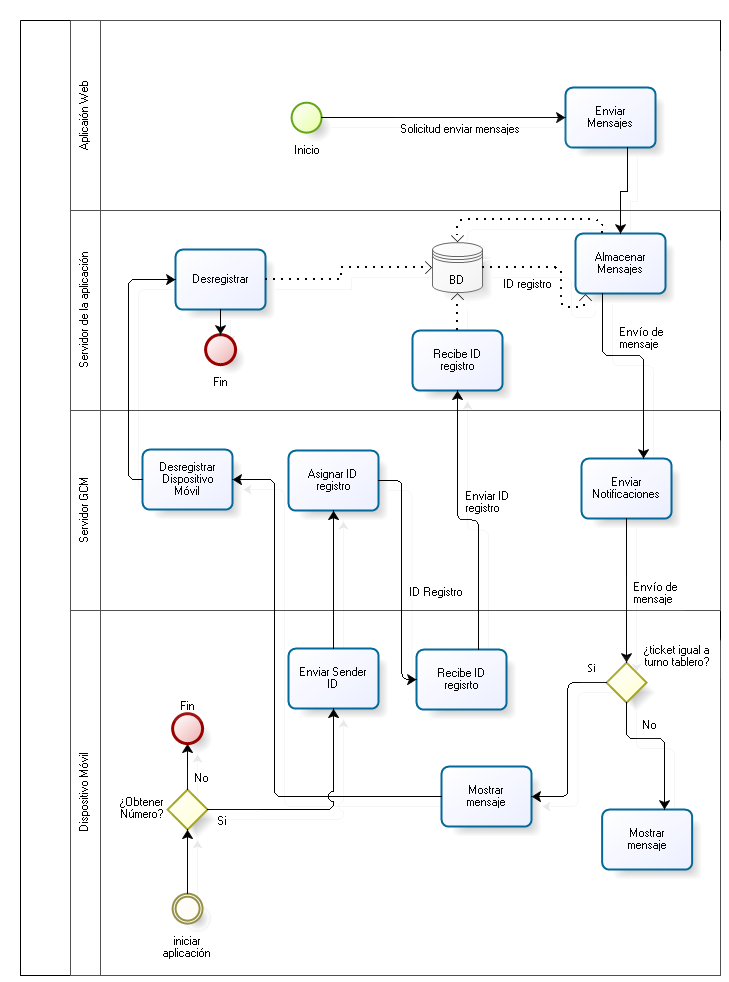
\includegraphics[scale=0.70]{images/capitulo4/diagramaProceso.png}
\caption{Diagrama de Proceso Aplicación Móvil.}
\label{diagramaProceso}
\end{figure}


\subsubsection{Modelo de Datos}

\begin{figure}[H]
\centering
\setlength\fboxsep{0pt}
\setlength\fboxrule{0.5pt}
\fbox{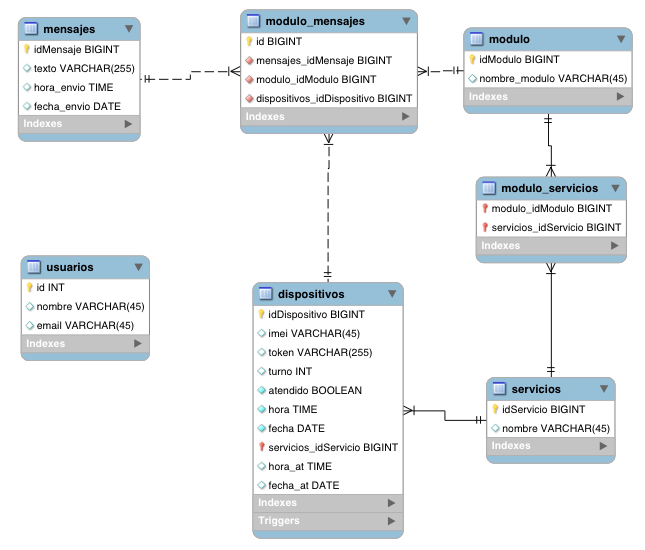
\includegraphics[scale=0.60]{images/capitulo4/modeloDatos.png}}
\caption{Modelo de datos.}
\label{modeloDeDatos}
\end{figure}

\myparagraph{Diccionario de datos}

\begin{spacing}{1.0}
	\begin{table}[H]
		\centering
		\caption{Diccionario de datos tabla ``dispositivos''.} 
		\begin{tabular}{|c|c|c|}
			\hline 
			\rowcolor{gray!30} &&\\
			\rowcolor{gray!30} \textbf{Columna} & \textbf{Tipo de dato} & \textbf{Descripción} \\ 
			\rowcolor{gray!30} &&\\
			\hline 
			&&\\[-0.2cm]
			idDispositivos & BIGINT & Identificador único de cada dispositivo. \\
			\hline 
			&&\\[-0.2cm]
			imei & VARCHAR(45) & Identificador propio de cada \textit{smartphone}. \\
			\hline 
			&&\\[-0.2cm]
			token & VARCHAR(255) & Identificador entregado por GCM a cada \\
			 & & dispositivo móvil registrado en el sistema. \\
			\hline 
			&&\\[-0.2cm]
			turno & INT & Número de turno de atención asignado \\
			 & & por el sistema a un dispositivo móvil. \\
			\hline 
			&&\\[-0.2cm]
			atendido & BOOLEAN & Estado de atención en que encuentra \\
			 & & un dispositivo, TRUE o FALSE. \\
			\hline 
			&&\\[-0.2cm]
			hora & TIME & Hora en que el dispositivo solicita un turno \\
			 & & de atención. \\
			\hline
			&&\\[-0.2cm]
			fecha & DATE & Fecha en que el dispositivo solicita un turno \\
			 & & de atención. \\
			\hline
			&&\\[-0.2cm]
			servicios\_idServicio & BIGINT & Clave foránea de la tabla servicios. \\
			\hline
			&&\\[-0.2cm]
			hora\_at & TIME & Hora en que el cliente es llamado para ser \\
			 & & atendido en un módulo de atención. \\
			\hline
			&&\\[-0.2cm]
			fecha\_at & DATE & Fecha en que el cliente es llamado \\
			 & & para ser atendido en un módulo de atención. \\
		    \hline
		\end{tabular}
		\label{diccionario_dispositivos}
	\end{table}
\end{spacing}

\begin{spacing}{1.0}
	\begin{table}[H]
		\centering
		\caption{Diccionario de datos tabla ``mensajes''.} 
		\begin{tabular}{|c|c|c|}
			\hline 
			\rowcolor{gray!30} &&\\
			\rowcolor{gray!30} \textbf{Columna} & \textbf{Tipo de dato} & \textbf{Descripción} \\ 
			\rowcolor{gray!30} &&\\
			\hline 
			&&\\[-0.2cm]
			idMensaje & BIGINT & Identificador único de cada mensaje. \\
			\hline 
			&&\\[-0.2cm]
			texto & VARCHAR(255) & Mensaje enviado desde el sistema \\
			 & & a cada \textit{smartphone}. \\
			\hline 
			&&\\[-0.2cm]
			hora\_envio & TIME & Hora en que se envió el mensaje. \\
			\hline 
			&&\\[-0.2cm]
			fecha\_envio & DATE & Fecha en que se envió el mensaje. \\
			\hline
		\end{tabular}
		\label{diccionario_mensajes}
	\end{table}
\end{spacing}

\begin{spacing}{1.0}
	\begin{table}[H]
		\centering
		\caption{Diccionario de datos tabla ``modulo''.} 
		\begin{tabular}{|c|c|c|}
			\hline 
			\rowcolor{gray!30} &&\\
			\rowcolor{gray!30} \textbf{Columna} & \textbf{Tipo de dato} & \textbf{Descripción} \\ 
			\rowcolor{gray!30} &&\\
			\hline 
			&&\\[-0.2cm]
			idModulo & BIGINT & Identificador único de cada \\
			 & & módulo de atención. \\
			\hline 
			&&\\[-0.2cm]
			nombre\_modulo & VARCHAR(45) & Nombre del módulo de atención. \\
			\hline 
		\end{tabular}
		\label{diccionario_modulo}
	\end{table}
\end{spacing}

\begin{spacing}{1.0}
	\begin{table}[H]
		\centering
		\caption{Diccionario de datos tabla ``servicios''.} 
		\begin{tabular}{|c|c|c|}
			\hline 
			\rowcolor{gray!30} &&\\
			\rowcolor{gray!30} \textbf{Columna} & \textbf{Tipo de dato} & \textbf{Descripción} \\ 
			\rowcolor{gray!30} &&\\
			\hline 
			&&\\[-0.2cm]
			idServicio & BIGINT & Identificador único de cada servicio. \\
			\hline 
			&&\\[-0.2cm]
			nombre & VARCHAR(45) & Nombre del servicio. \\
			\hline 
		\end{tabular}
		\label{diccionario_servicios}
	\end{table}
\end{spacing}

\begin{spacing}{1.0}
	\begin{table}[H]
		\centering
		\caption{Diccionario de datos tabla ``usuarios''.} 
		\begin{tabular}{|c|c|c|}
			\hline 
			\rowcolor{gray!30} &&\\
			\rowcolor{gray!30} \textbf{Columna} & \textbf{Tipo de dato} & \textbf{Descripción} \\ 
			\rowcolor{gray!30} &&\\
			\hline 
			&&\\[-0.2cm]
			id & INT & Identificador único de cada usuario. \\
			\hline 
			&&\\[-0.2cm]
			nombre & VARCHAR(45) & Nombre y apellido del usuario. \\
			\hline
			&&\\[-0.2cm]
			email & VARCHAR(45) & Correo electrónico del usuario. \\
			\hline 
		\end{tabular}
		\label{diccionario_usuarios}
	\end{table}
\end{spacing}

\begin{spacing}{1.0}
	\begin{table}[H]
		\centering
		\caption{Diccionario de datos tabla ``modulo\_mensajes''.} 
		\begin{tabular}{|c|c|c|}
			\hline 
			\rowcolor{gray!30} &&\\
			\rowcolor{gray!30} \textbf{Columna} & \textbf{Tipo de dato} & \textbf{Descripción} \\ 
			\rowcolor{gray!30} &&\\
			\hline 
			&&\\[-0.2cm]
			id & BIGINT & Identificador único de la tabla. \\
			\hline 
			&&\\[-0.2cm]
			mensajes\_idMensaje & BIGINT & Identificador único de cada mensaje. \\
			\hline
			&&\\[-0.2cm]
			modulo\_idModulo & BIGINT & Identificador único de cada \\
			 & & módulo de atención. \\
			\hline
			&&\\[-0.2cm]
			dispositivos\_idDispositivos & BIGINT & Identificador único de cada dispositivo. \\
			\hline 
		\end{tabular}
		\label{diccionario_servicios}
	\end{table}
\end{spacing}

\begin{spacing}{1.0}
	\begin{table}[H]
		\centering
		\caption{Diccionario de datos tabla ``modulo\_servicios''.} 
		\begin{tabular}{|c|c|c|}
			\hline 
			\rowcolor{gray!30} &&\\
			\rowcolor{gray!30} \textbf{Columna} & \textbf{Tipo de dato} & \textbf{Descripción} \\ 
			\rowcolor{gray!30} &&\\
			\hline 
			&&\\[-0.2cm]
			modulo\_idModulo & Identificador único de cada \\
			 & & módulo de atención. \\
			\hline 
			&&\\[-0.2cm]
			servicios\_idServicios & BIGINT & Identificador único de cada servicio. \\
			\hline
		\end{tabular}
		\label{diccionario_servicios}
	\end{table}
\end{spacing}



